\subsection{DSPIGCN}
\label{sec:dspigcn}
\paragraph{Implementation and independence.}
YAN Zhengyang's implementation follows the dual-stream architecture of
Guo et al.~\cite{guo2026dspigcn}. Separate displacement and velocity branches
combine four-head temporal attention, a symmetrically normalized graph
convolution and a residual causal temporal convolution. Four-layer decoders
produce bivariate Gaussian position parameters and velocities. A four-layer
convolutional network estimates a degree-four polynomial, whose analytic
derivative couples the two branches. The loss combines Gaussian negative
log-likelihood, squared reconstruction error and the position/velocity
physical residual, with physics weight 0.1. All model, loss, trainer and
sampler code was written for this project with acknowledged Codex assistance;
only the group's neutral loader, corruption and evaluator are shared.

\paragraph{Registered departures.}
The implementation uses target-centered metric positions, seconds-based
velocities, a 3 m history-only neighbor filter, and residual initialization
around the last observed velocity. Gaussian means represent displacement
from the forecast origin rather than per-step increments. Polynomial
coefficients are rescaled from normalized time to physical seconds before
differentiation. Algorithm 2 is implemented as a stratified equal-weight
mixture over forecast times, followed by nearest-unused-anchor assignment.
The consulted public reference differs from the paper in reconstruction and
sampling; our source notes identify the exact version and discrepancies.
These choices preclude claiming exact reproduction of the published scores.

\paragraph{Verification and selection.}
The target and neighbor feature tests change future coordinates, future
neighbor availability and supplied derivative columns without changing model
inputs. Additional checks cover metric round trips, derivative units,
polynomial gradients, analytic likelihood, graph padding/permutation,
seeded sample conservation and optimization through all branches. The formal
configuration specifies all five holdouts, seeds 0--2, 200 SGD epochs and
batch size 128. Checkpoints are selected every ten epochs using clean
validation Energy Score, then mean ADE and earlier epoch. One selected
checkpoint generates all six conditions; no test result enters selection.

\paragraph{Accuracy and robustness.}
Each of the 34,161 target windows receives 20 sampled paths. On clean inputs,
minADE and minFDE were \ModelMetric{dspigcn}{clean_0}{min_ade_mean} and
\ModelMetric{dspigcn}{clean_0}{min_fde_mean}\,m. The corresponding mean errors
were \ModelMetric{dspigcn}{clean_0}{mean_ade_mean} and \ModelMetric{dspigcn}{clean_0}{mean_fde_mean}\,m.
The Energy Score was \ModelMetric{dspigcn}{clean_0}{energy_score_mean}\,m.
The clean mean ADE ranged from 0.602 m on ZARA2 to 1.200 m on ETH. Each holdout has equal weight. Mean ADE was 2.716 m with 0.20 m target-history noise and 0.912 m after filling two missing observations.

\begin{figure}[htbp]
\centering
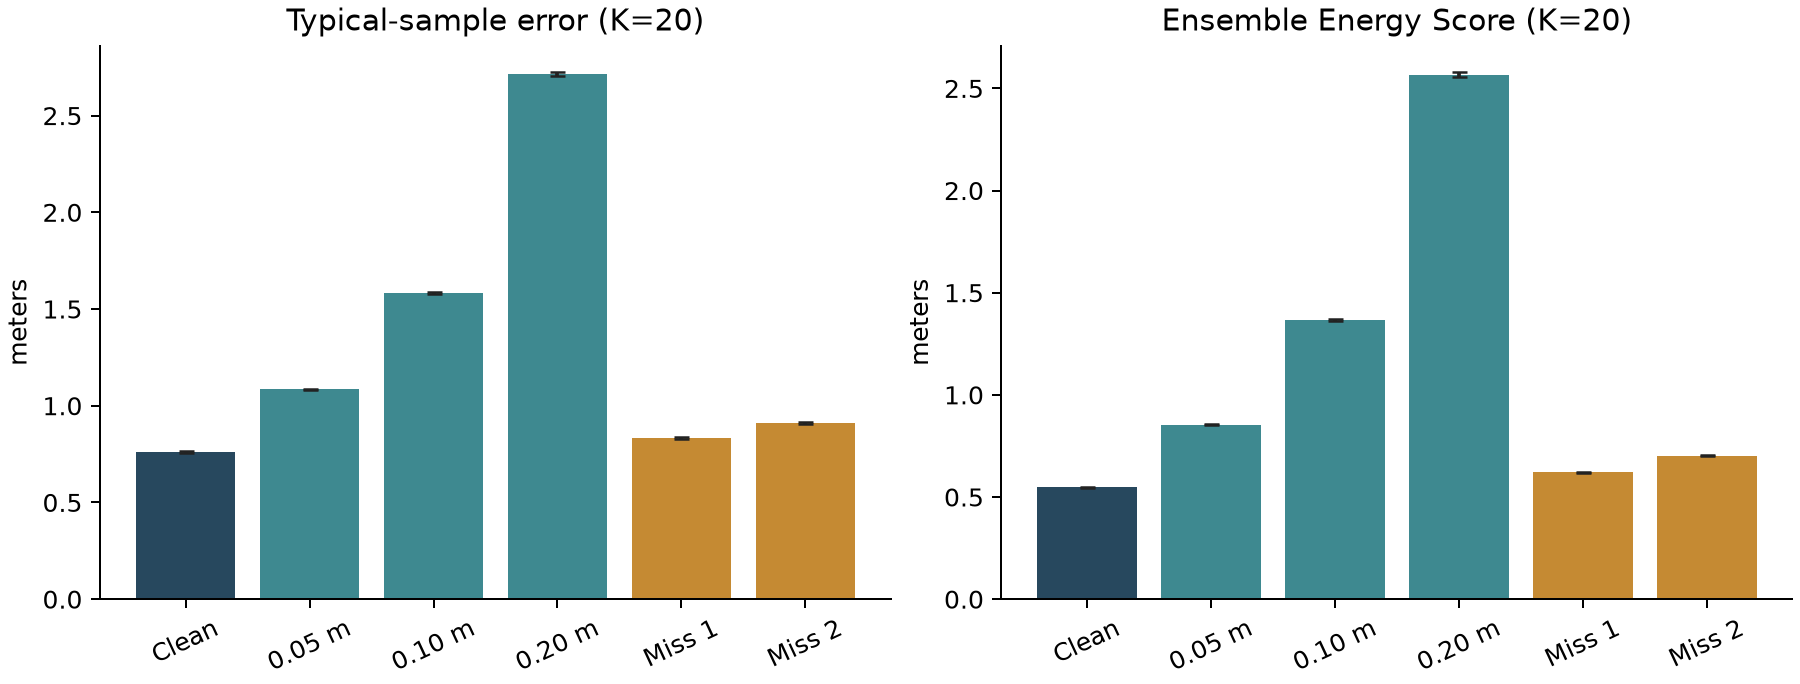
\includegraphics[width=.91\linewidth,height=2.05in,keepaspectratio]{contributions/dspigcn/assets/robustness.png}
\caption{DSPIGCN across the six common conditions. Bars give equal-weight scene means and error bars give the standard deviation of three seed means.}
\label{fig:dspigcn-robustness}
\end{figure}

\paragraph{Motion, examples and runtime.}
Clean sampled steps changed direction by 76.0 degrees on average. Each adjacent step had to exceed 0.05 m/s to enter this calculation. The largest clean mean ADE at seed zero was 5.539 m on ETH, where the target had 2 visible neighbors. The five fixed examples were chosen from the shared runtime list before the errors were inspected. On the fixed ETH window, mean ADE was 0.989 m with clean observations, 0.974 m with noise and 3.703 m with two missing observations.
The within-window 99th percentile of predicted acceleration exceeded its training threshold in 99.6\% of clean windows and 100.0\% with 0.20 m position noise. These percentages give each holdout equal weight.
End-to-end latency was \ModelRuntime{dspigcn}{end_to_end_ms}\,ms for 128 targets on NVIDIA GeForce RTX 4090, using the median of 15 run medians. This measurement includes visible-neighbor discovery, prediction, anchor sampling and transfer to the CPU. The physical loss constrains the predicted means during training. Its contribution to accuracy would require a separate ablation. The sampler assigns anchors without replacement, so its twenty trajectories are dependent. The Energy Score summarizes this ensemble; the standard deviations across three seeds describe variation between fits.
